
%(BEGIN_QUESTION)
% Copyright 2010, Tony R. Kuphaldt, released under the Creative Commons Attribution License (v 1.0)
% This means you may do almost anything with this work of mine, so long as you give me proper credit

Nivåreguleringen på denne steam kokeren har et problem. Vannivået i steambeholderen er under settpunktet. Regulatoren viser en PV på 42\% med et settpunkt på 50\%. Det har vert slik i flere timer, til tross for at operatøren har forsøkt å endre settpunkt. Kokeren går for fult og lager steam som normalt. 

%This boiler steam drum level control system has a problem.  The water level in the steam drum is below setpoint (as indicated by the controller display showing 42\% water level with a 50\% setpoint), and has been for the past several hours despite the operator's attempt to raise water level by raising the setpoint on the controller.  Meanwhile, the boiler is operating at full power, making steam at a normal rate of flow:

$$\includegraphics[width=15.5cm]{i01368x01.eps}$$

Identifiser sannsynligheten for hver av de spesifiserte feilene nedenfor. Du skal bare ta hensyn til en feil av gangen(ingen dobbeltfeil). Finn ut om hver av feilene kan være ansvarlig for symptomene i dette systemet. 

%Identify the likelihood of each specified fault for this system.  Consider each fault one at a time (i.e. no coincidental faults), determining whether or not each fault could independently account for {\it all} measurements and symptoms in this system.

% No blank lines allowed between lines of an \halign structure!
% I use comments (%) instead, so that TeX doesn't choke.

$$\vbox{\offinterlineskip
\halign{\strut
\vrule \quad\hfil # \ \hfil & 
\vrule \quad\hfil # \ \hfil & 
\vrule \quad\hfil # \ \hfil \vrule \cr
\noalign{\hrule}
%
% First row
{\bf Feil} & {\bf Mulig} & {\bf Umulig} \cr
%
\noalign{\hrule}
%
% Another row
LT kalibreringsfeil &  &  \cr
%
\noalign{\hrule}
%
% Another row
LY Kalibreringsfeil &  &  \cr
%
\noalign{\hrule}
%
% Another row
Defekt regulator &  &  \cr
%
\noalign{\hrule}
%
% Another row
Lavt trykk på luftforsyning &  &  \cr
%
\noalign{\hrule}
%
% Another row
Unormalt stor motstand i LT strømsløyfe &  &  \cr
%
\noalign{\hrule}
%
% Another row
Unormalt stor motstand i LY strømsløyfe &  &  \cr
%
\noalign{\hrule}
%
% Another row
Feedwater pumpe er slitt &  &  \cr
%
\noalign{\hrule}
%
% Another row
Regulatoren står i manuell modus. &  &  \cr
%
\noalign{\hrule}
} % End of \halign 
}$$ % End of \vbox

\underbar{file i01368}
%(END_QUESTION)





%(BEGIN_ANSWER)

Students are often surprised to find that a transmitter calibration error would {\it not} cause this problem.  A calibration error in the LT {\it would} cause the actual steam drum level to drift off setpoint, but with this being the only problem the controller would still register right on setpoint!

\vskip 10pt

A vital ``next test'' is to check the controller output, to see what it is trying to tell the valve to do.  It {\it should} be commanding the valve to open up.  If not, the controller definitely has some sort of problem (or is in manual mode).

%(END_ANSWER)





%(BEGIN_NOTES)

% No blank lines allowed between lines of an \halign structure!
% I use comments (%) instead, so that TeX doesn't choke.

$$\vbox{\offinterlineskip
\halign{\strut
\vrule \quad\hfil # \ \hfil & 
\vrule \quad\hfil # \ \hfil & 
\vrule \quad\hfil # \ \hfil \vrule \cr
\noalign{\hrule}
%
% First row
{\bf Fault} & {\bf Possible} & {\bf Impossible} \cr
%
\noalign{\hrule}
%
% Another row
LT calibration error &  & $\surd$ \cr
%
\noalign{\hrule}
%
% Another row
LY calibration error & ? &  \cr
%
\noalign{\hrule}
%
% Another row
Controller failed & $\surd$ &  \cr
%
\noalign{\hrule}
%
% Another row
Low air supply pressure & $\surd$ &  \cr
%
\noalign{\hrule}
%
% Another row
Excessive resistance in LT circuit &  & $\surd$ \cr
%
\noalign{\hrule}
%
% Another row
Excessive resistance in LY circuit &  & $\surd$ \cr
%
\noalign{\hrule}
%
% Another row
Feedwater pump worn & $\surd$ &  \cr
%
\noalign{\hrule}
%
% Another row
Controller in manual mode & ? &  \cr
%
\noalign{\hrule}
} % End of \halign 
}$$ % End of \vbox

An LY calibration error is possible only if the error is quite significant.  Otherwise, the controller will compensate for any modest valve errors through feedback.

The ``excessive resistance'' faults are not possible if we assume the extra resistance to be insufficient to cause the controller or transmitter to saturate.  Ideally, both current sources (LT and LIC) will fight as hard as they must to maintain proper current in each circuit, even with extra resistance.  However, if the extra resistance is very large, it would be possible for that resistance to force either current value to be less than it should be.

A controller in manual usually does not allow changes in setpoint due to the standard ``setpoint tracking'' feature.  If this feature is turned off, however, changes in setpoint are possible in manual mode.

\vskip 20pt \vbox{\hrule \hbox{\strut \vrule{} {\bf Virtual Troubleshooting} \vrule} \hrule}

This question is a good candidate for a ``Virtual Troubleshooting'' exercise.  Presenting the diagram to students, you first imagine in your own mind a particular fault in the system.  Then, you present one or more symptoms of that fault (something noticeable by an operator or other user of the system).  Students then propose various diagnostic tests to perform on this system to identify the nature and location of the fault, as though they were technicians trying to troubleshoot the problem.  Your job is to tell them what the result(s) would be for each of the proposed diagnostic tests, documenting those results where all the students can see.

During and after the exercise, it is good to ask students follow-up questions such as:

\begin{itemize}
\item{} What does the result of the last diagnostic test tell you about the fault?
\item{} Suppose the results of the last diagnostic test were different.  What then would that result tell you about the fault?
\item{} Is the last diagnostic test the best one we could do?
\item{} What would be the ideal order of tests, to diagnose the problem in as few steps as possible?
\end{itemize}

%(END_NOTES)


